\chapter{Исследовательская часть}

В данном разделе будут приведены результаты работы разработанного программного обеспечения и поставлен эксперимент по сравнению уровня и характера шума синтезируемого изображения с использование классическом алгоритма (метода Монте - Карло) и квантового алгоритма избыточной выборки на различных размерах изображения.

\section{Результаты работы программного обеспечения}

% 3, 4, 5
На изображении \ref{img:example_01} приведен результат работы программы с размером синтезируемого изображения 512x512 пикселей и при использовании 4 итераций увеличения комплексной амплитуды. 

\begin{figure}[H]
	\begin{center}
		%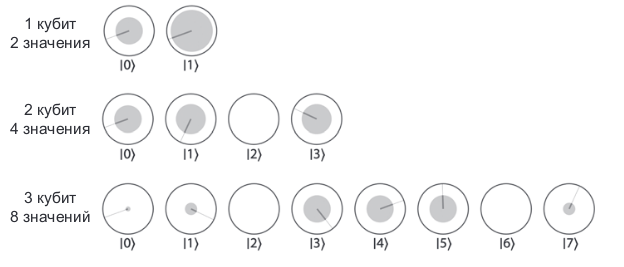
\includegraphics[scale=0.7]{img/qint.png}
	\end{center}
	\captionsetup{justification=centering}
	\caption{Результаты работы ПО с размером синтезируемого изображения 512х512 и использования 4 итераций увеличения комплексной амплитуды}
	\label{img:example_01}
\end{figure}

На рисунке \ref{img:example_02} представленно тоже самое изображение, но уже при использовании 8 итераций увеличения комплексной амплитуды. 

\begin{figure}[H]
	\begin{center}
		%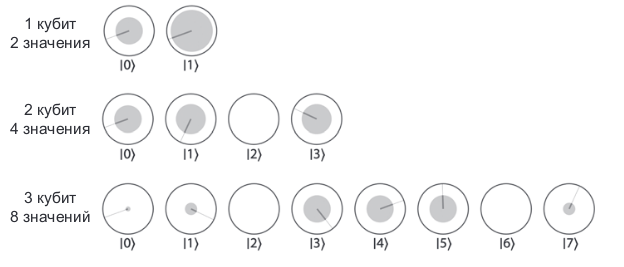
\includegraphics[scale=0.7]{img/qint.png}
	\end{center}
	\captionsetup{justification=centering}
	\caption{Результаты работы ПО с размером синтезируемого изображения 512х512 и использования 8 итераций увеличения комплексной амплитуды}
	\label{img:example_02}
\end{figure}

\begin{figure}[H]
	\begin{center}
		%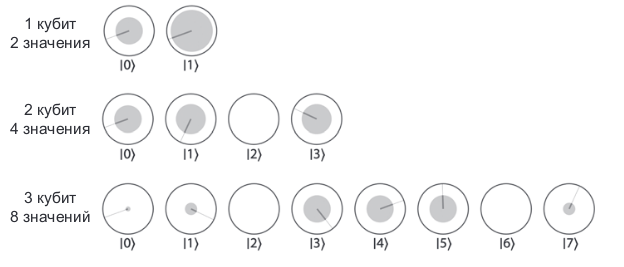
\includegraphics[scale=0.7]{img/qint.png}
	\end{center}
	\captionsetup{justification=centering}
	\caption{Результаты работы ПО с размером синтезируемого изображения 1024х1024 и использования 4 итераций увеличения комплексной амплитуды}
	\label{img:example_03}
\end{figure}

На риснуке \ref{img:example_03} представлен результат работы программы при синтезе изображения размером 1024х1024 пикселя и при использовании 4 итераций усиления комплексной амплитуды.

\section{Постановка эксперимента} 

\subsection{Цель эксперимента}

Целью эксперимента является проведение сравнения уровня и характера зашумлённости изображения синтезируемого классическим алгоритмом избыточной выборки (алгоритм Монте-Карло) и алгоритмом квантовой избыточной выборки.

\subsection{Описание эксперимента}

Сравнить уровень зашумленности двух синтезируемых изображений можно методом основанным на оценке отклонения от медианы \cite{noise}. Вычисление в этом методе выполняется в два этапа. На первом этапе вычисляют отклонение от медианы для каждого пикселя всего изображения, по формуле (\ref{for:noise_01}):

\begin{equation} 
	\label{for:noise_01}
	MAD(i, j) = I(i, j) - median(I(i, j))
\end{equation}
где $I(i, j)$ -- отсчёт, описывающий пиксель с координатами $i$, $j$.

На втором этапе вычисляется медиана для всего массива и умножается на полученный опытным путём коэффициент (\ref{for:noise_02}):

\begin{equation} 
	\label{for:noise_02}
	Nrms = 1.483 * median(MAD)
\end{equation}
Результатом расчёта является среднеквадратическое значение шума $Nrms$.

Результаты сравнения уровня зашумлённости для изображений разных размеров приведены в таблице 4.1. Во втором и третьем столбце таблицы расположено среднеквадратическое значение шума $Nrms$ для рассматриваемых реализаций алгоритмов.

\begin{table}[h!]
	\label{tab:noise}
	\caption{Сравнение уровня зашумленности для классического и квантового алгоритма избыточной выборки.}
	\begin{center}
		\begin{tabular}{|c c c|} 
			\hline
			Размер изображения & Классическая выборка & Квантовая выборка \\  
			\hline
			64x64 &  &   \\
			\hline
			128x128 &  &  \\
			\hline
			256x256 &  &   \\
			\hline
			512x512 &  & \\
			\hline
			1024x1024 &   & \\
			\hline
		\end{tabular}
	\end{center}
\end{table}

Сравнение характера шума синтезируемого изображения размером 1024x1024 приведено на рисунке \ref{img:noise}.

\begin{figure}[h!]
	\begin{center}
		%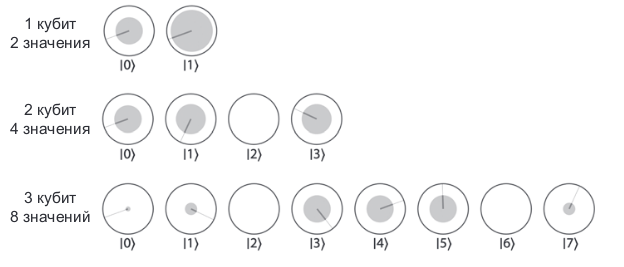
\includegraphics[scale=0.7]{img/qint.png}
	\end{center}
	\captionsetup{justification=centering}
	\caption{Сравнение характера шума полученного изображения. Первое изображение -- идеальное, второе -- классический алгоритм, третье -- квантовый алгоритм}
	\label{img:noise}
\end{figure}


\section*{Вывод}

тут вывод по таблице и картинке